% -*- coding: utf-8 -*-

\section{Introduction}
\label{introduction}



The area of protein folding (and from this the creation of newer and better drugs) with the aid of computers, has since the 60's been an area of great research and experimentation. 


The influence of computers in modern medicine is becoming increasingly important. In order to find new and better drugs scientists have turned to computer in order to simulate human biology.

An often used method is protein folding, where different foldings of proteins are tested for interesting properties. Since proteins cannot physically overlap with another part, the program has to check whether there is a collision or not. Since this test has to be done often, it is critical that the overlap tests can be done fast. 

One method for detecting collisions is Bounding Volumes Hierarchy (BVH), using a Bounding Volume (BV), where each node in the BVH is enveloped by a BV that covers the all children of the nodes (with the leafs of the node being parts of the protein itself). If a BV does not intersect any other BV, then it is clear that the attempted fold is legal, and it can take place. If there is a collision between two or more BVs, then further checks are needed, in order to check whether there truly is an overlap.

\begin{figure}
\centering
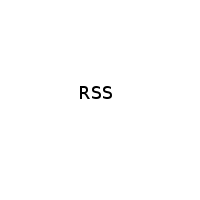
\includegraphics[width=0.5\textwidth]{figures/rss}
\caption{\label{rss-example-figure}An example of a RSS}
\end{figure}

One of possible BV is the Rectangular Swept Sphere (RSS), which is generated by sweeping a sphere (with a positive radius) over a rectangle in 3D space. The resulting volume looks something like a pillow - see figure \ref{rss-example-figure}. 

I will in this project attempt to implement a reasonably effective RSS BV, with the ability to test for overlap detection, the ability to create a new RSS from a set of points, and the ability to crate a new RSS that contains all the points of 2 (possibly distinct) RSS'.

\subsection{Scope and Limitations}
\label{scope}
I will not try to implement the RSS in the BVH, and as a consequence not perform tests on it based on active folding of proteins, though I will test it on provided test data derived from snapshots of protein foldings.

\subsection{Expectations to the reader}
I expect the reader to have a good grasp of computational geometry and, vector manipulations and algorithms in general.

\subsection{Terminology}

\subsection{Guide to this report}
\begin{description}
\item[Section \ref{introduction}] The introduction to the report, which will introduce the subject and explain my goals
\item[Section \ref{rss}] A description of the Rectangular Swept Spheres - how they are defined in theory, and how I have chosen to represent them. This section will also contain information about some of the literature that has worked with RSS.
\item[Section \ref{algorithms}] The algorithms that work on the RSSs, and an analysis of their run time 
\item[Section \ref{implementation}] Notes on the implementation of the algorithms from the previous section and the RSS itself in ProGAL.
\item[Section \ref{results}] A discussion about the results of the implementation together with a comparison with Oriented Bounding Boxes. 
\item[Section \ref{conclusion}] The conclusion of the report, where I will sum up the findings 
\end{description}

\subsection{Literature used in this report}
For this project I have used the following literature: \Sfixme{find out whether it should be here, or in section 2}
\begin{description}
\item[\cite{larsen00fast}] Gives an introduction to some of the problems with making Distance Queries between RSSs. The article refers \cite{Larsen99fastproximity} (by the same authors) which contains more explicit information on how to calculate the distance. 
\item[\cite{Lotan03algorithmand}] Gives a general introduction to Monte Carlo simulation of Proteins, as well as a comparison of several data-structures and algorithms for these, for protein folding. None of the material in this article is used directly, but rather as background material.
\item[\cite{Larsen99fastproximity}] A more in-depth description of how the distance queries for the RSSs can be preformed. However, it leaves the most difficult cases to \cite{237244}.
\item[\cite{237244}] A description the algorithm for the most difficult case of RSS distance query. Although the algorithm as described is for Oriented Bounding Boxes (OBB).
\end{description}

\Sfixme{Make introduction conclusion}
